\chapter{Funktionstest}
Nach der Implementierung des zuvor geschilderten Konzepts wurde ein Funktionstest durchgeführt.
Dazu werden zunächst die theoretischen Grenzen der Konfiguration getestet und danach die tatsächlichen Ausgabewerte mit den theoretischen verglichen.
Besonders interessant ist hierbei, in welchem Frequenzbereich der Generator zuverlässig funktioniert.

\section{theoretische Limitierungen}
Um den praktischen Nutzen des Funktionsgenerators einzuschätzen, werden die Grenzen der einstellbaren Frequenz, die Auflösung und der Spannungsbereich berechnet.
Für die Spannung ergeben sich diese Werte aus dem Datenblatt des eingesetzten DACs, dieser kann in einem Bereich von 0 bis 5,5 V eingesetzt werden, wobei die Referenzspannung 2,7 V nicht unterschreiten darf \cite{PmodDA2}.
Für den Betrieb auf dem Basys 3 Board läuft der Spannungsbereich von 0 bis 3,3 V, da hier die Ausgangsspannung des Boards der limitierende Faktor ist.
Nachfolgend werden noch der Frequenzbereich und die Auflösung bestimmt.

\subsection{Frequenzbereich}
Der Systemtakt $f_{sys}$ des Generators beträgt 100 MHz.
Der Frequenzbereich der Funktionen, die er ausgeben kann, reicht von ca. 0,0877 Hz bis zu ca. 735 kHz.
Die Frequenz $f_{count}$ ist die Frequenz mit der der interne Zähler der Funktionsbausteine hochzählt und beträgt ein 64tel des Systemtakts $f_{sys}$ (siehe \cref{test:theo:freq:fcount}).
Die minimale Frequenz $f_{min}$ errechnet sich aus dem maximalen Zählstand, der wiederum abhängig ist von seiner Bitbreite \code{clk\_width} (siehe \cref{test:theo:freq:fmin}).
Die maximale Frequenz ergibt sich aus dem Shannon'schen Abtasttheorem, nach dem die minimale Abtastfrequenz eines Signals doppelt so groß sein muss, wie die Frequenz des abgetasteten Signals \cite(blabla).
In diesem Fall entspricht die Abtastfrequenz $f_{count}$ und das abgetastete Signal dem Ausgangssignal, woraus folgt, dass das ausgehende Signal nur halb so groß sein kann, wie $f_{count}$ (siehe \cref{test:theo:freq:fmin}).

\begin{align}
  f_{count} &= \frac{f_{sys}}{68} \label{test:theo:freq:fcount}\\  
  f_{max} &= \frac{f_{count}}{2}  \label{test:theo:freq:fmax}\\ 
  f_{min} &= \frac{f_{count}}{2^{clk\_width} - 1} \label{test:theo:freq:fmin}
\end{align}

\subsection{Auflösung}
Die Auflösung des analogen Ausgangssignals hängt sowohl von der Geschwindigkeit ab, mit der das digitale Signal analogisiert werden kann, als auch von der maximalen Anzahl digital darstellbarer Werte.
Überschreitet die Frequenz des analogen Signals $f$ die Grenzfrequenz $f_{grenz}$, so fällt die Auflösung $R$ reziprok zu $f$ ab (siehe \cref{test:theo:res:plot}).
Oberhalb von $f_{grenz}$ ist die Auflösung durch die Bitbreite des ADCs begrenzt.
Da es sich um einen 12-Bit Wandler handelt, beträgt die Anzahl darstellbarer Werte und damit auch die höchste Auflösung $2^{12} = 4096$.
Diesen Wert nimmt die Auflösung an, wenn die Frequenz kleiner als $f_{grenz}$ ist (siehe \cref{test:theo:freq:fgrenz}).

\begin{align}
  R &= \begin{cases}
    4095               & f \leq f_{grenz}                      \\
    \frac{f_{count}}{f} & f > f_{grenz} = \frac{f_{count}}{4095} = 359 Hz
        \end{cases} \label{test:theo:freq:fgrenz}
\end{align}

Konkret bedeutet dass für den Funktionsgenerator, dass bei einer Amplitude von $U_{SS}=3,3V$ und einer Frequenz von $f=100kHz$, die Auflösung $4,54V^{-1}$ statt der maximalen Auflösung von $1241V^{-1}$ beträgt, das heißt, dass bei 100kHz 4,54 Werte statt 1241 Werte pro Volt gesampelt werden.

\begin{figure}[h] \centering
    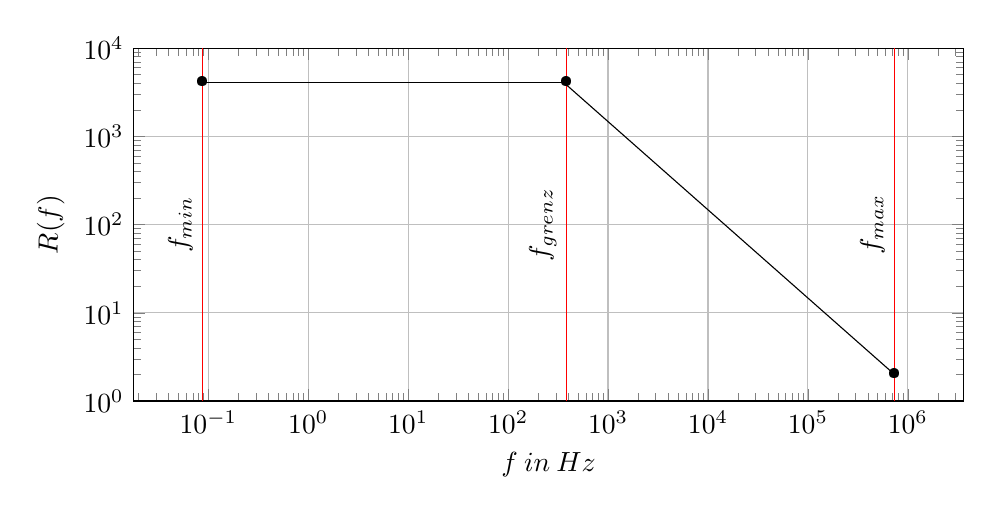
\begin{tikzpicture}
      \begin{loglogaxis}
        [xlabel=$f\:in\:Hz$,
        ylabel=$R(f)$,
        ymin=1,
        ymax=10000,,
        width=\textwidth,
        height=0.5\textwidth,
        grid=major]
        \addplot[color=black, domain=0.08765:359.12] {4095};
        \addplot[color=black, domain=359.12:735294] {100000000 / (68*\x)};
        % help lines and nodes:
        \addplot[color=red] coordinates{(381.12, 1)(381.12, 10000)};
        \node[above, rotate=90] at (381.12, 100) {$f_{grenz}$};
        \node at (381.12, 4095) {\textbullet};

        \addplot[color=red] coordinates{(0.08765, 1)(0.08765, 10000)};
        \node[above, rotate=90] at (0.08765, 100) {$f_{min}$};
        \node at (0.08765, 4095) {\textbullet};

        \addplot[color=red] coordinates{(735294, 1)(735294, 10000)};
        \node[above, rotate=90] at (735294, 100) {$f_{max}$};
        \node at (735294, 2) {\textbullet};
      \end{loglogaxis}
    \end{tikzpicture}
 \caption{Doppelt logarithmisches Diagramm der Auflösung $R(f)$ über den Frequenzbereich $f$. Die Auflösung bleibt konstant bei 4095 1/tick bis sie schließlich bei $f_{grenz}$ anfängt zu sinken.} \label{test:theo:res:plot}
\end{figure}

\section{reales Verhalten}
Nun soll das reale Verhalten des Funktionsgenerators untersucht werden.

\subsection{Versuchsaufbau}
Ein Foto des Versuchsaufbaus findet sich in \cref{test:real:setup:pic}.
Das digitale Oszilloskop Analog Discovery 2 von digilent wird dazu an einen Laptop angeschlossen, auf dem dann die Funktionsverläufe angezeigt werden.

\begin{figure}[h]
  \includegraphics[width=\textwidth]{testaufbau_fg}
  \caption{Versuchsaufbau zum Testen des Funktionsgenerators. Das Oszilloskopist mittels des Moduls Discovery BNC an den analog Ausgang des PmodDA2-Wandlers angeschlossen. Das Basys 3-Board wird über das angeschlossene USB Kabel mit Strom versorgt und per UART konfiguriert. Die vom Oszilloskop eingelesenen Daten werden an einen per USB angeschlossenen Laptop verschickt. Die LEDs auf dem Board zeigen den internen digitalen Funktionswert an.} \label{test:real:setup:pic}
\end{figure}

\subsection{Versuchsdurchführung}
Um zunächst die korrekte Ausgabe der Funktionsverläufe zu überprüfen, werden alle vier Verläufe nacheinander bei konstanter Frequenz $f=100Hz$ über die UART-Schnittstelle konfiguriert und die erfassten Signale dokumentiert.
Anschließend werden alle Funktionen der UART-Schnittstelle überprüft, indem der jeweilige Befehl mit einem dazu passenden Argument abgeschickt wird.
Schließlich wird noch der Frequenzbereich anhand der Zick-Zack-Funktion untersucht.
Dazu wird ein Wert knapp unterhalb von $f_{min}$ und ein Wert oberhalb von $f_{max}$ eingestellt.
Dazwischen wird, von 0.1 Hz aufwärts, mit jedem Schritt die eingestellte Frequenz mit 10 multipliziert.
Auffäligkeiten im Funktionsverlauf werden festgehalten.

\subsection{Ergebnis}

\begin{figure}[h] \centering
  {
    \pgfplotsset{
    no markers,
    grid=major,
    ymin=-0.2, ymax=3.5,
    width=0.5\textwidth}
  % constant
  \subfloat[][konstante Funktion]{ 
    \begin{tikzpicture}
      \begin{axis}[ylabel=$U(t)$]
        \addplot table [x=Time (s), y=Channel 2 (V), col sep=comma, row sep=newline] {test/const100Hz_small.csv};
      \end{axis}
    \end{tikzpicture}
    \label{test:real:res:plot:const}
  } 
  % square
  \subfloat[][Rechteckfunktion]{
    \begin{tikzpicture}
      \begin{axis}
        \addplot table [x=Time (s), y=Channel 2 (V), col sep=comma, row sep=newline] {test/square100Hz_small.csv};
      \end{axis}
    \end{tikzpicture}
    \label{test:real:res:plot:square}
  } 

  % zigzag \foreach \x in {0, 15, ..., 90} {(\x, 3.3)}
  \subfloat[][Zick-Zack-Funktion]{
    \begin{tikzpicture}
      \begin{axis}[ylabel=$U(t)$, xlabel=$t$]
        \addplot table [x=Time (s), y=Channel 2 (V), col sep=comma, row sep=newline] {test/zigzag100Hz_small.csv};
      \end{axis}
    \end{tikzpicture}
    \label{test:real:res:plot:zigzag}
  }
  % ramp
  \subfloat[][Rampenfunktion]{
    \begin{tikzpicture}
      \begin{axis}[xlabel=$t$]
        \addplot table [x=Time (s), y=Channel 2 (V), col sep=comma, row sep=newline] {test/ramp100Hz_small.csv};
      \end{axis}
    \end{tikzpicture}
    \label{}
  }
}
  \caption{Die Ergebnisse des Versuchs bei $f=100Hz$. } \label{test:real:res:plot}
\end{figure}

% auswertung
\subsection{Auswertung}

